% @TODO Change this
\chapter{Contour Trees}
\label{chapter3}

% @TODO Add quote reeb graph intro.
The Reeb graph of a scalar field is connected and acyclic \cite{comp-topo}. As such we will call the Reeb graph of a scalar field the contour tree. In this chapter we will assemble the theory we have presented thus far and use it to introduce the state of the art serial and parallel algorithms for contour tree computation. We will begin with a short discussion on how we treat input data and what theoretical simplifying assumptions we are making. Afterwards we will present an overview of contour tree algorithms and then introduce some graph theoretical properties of contour trees. Next we will describe in detail how the serial and parallel contour tree algorithm work. This will lead us to defining the so called w-structures. We will demonstrate why exactly they are a pathological case that causes poor performance in the parallel contour tree algorithm. The final topic of this chapter is contour tree simplification. This is the process of identifying and removing parts of the contour tree that are not topologically significant.

\section{Typical Input Data}

% @TODO Add this back if you have the time.

% Such a process is for example the sampling of temperature from a bounded volume of air [] or the height of points over a geographic region []. The contour tree is shown to be a robust tool primarily used in the visualisation of such natural phenomena [].

Many scientific and medical applications require the sampling of scalar values from a bounded area or volume in two or three dimensional Euclidean space \cite{carr-masters}. The theory we have presented so far is applicable only in the continuous setting but the resolution of any sampling process is finite. If we are to leverage this theory we must assume an underlying continuous function in the whole of the area or volume and not just at the sampled points. To do so we will construct an approximation of this function based on the values we have sampled. This is usually done by constructing a simplicial complex where the data points are the vertices and higher dimensional simplicies are added to completely fill the space between them (see Figure \ref{fig:simplicial-mesh}). We will call the resulting data structure a simplical mesh \cite{carr-masters}.

\begin{figure}[h]%
    \centering
    \subfloat[Input Data]{{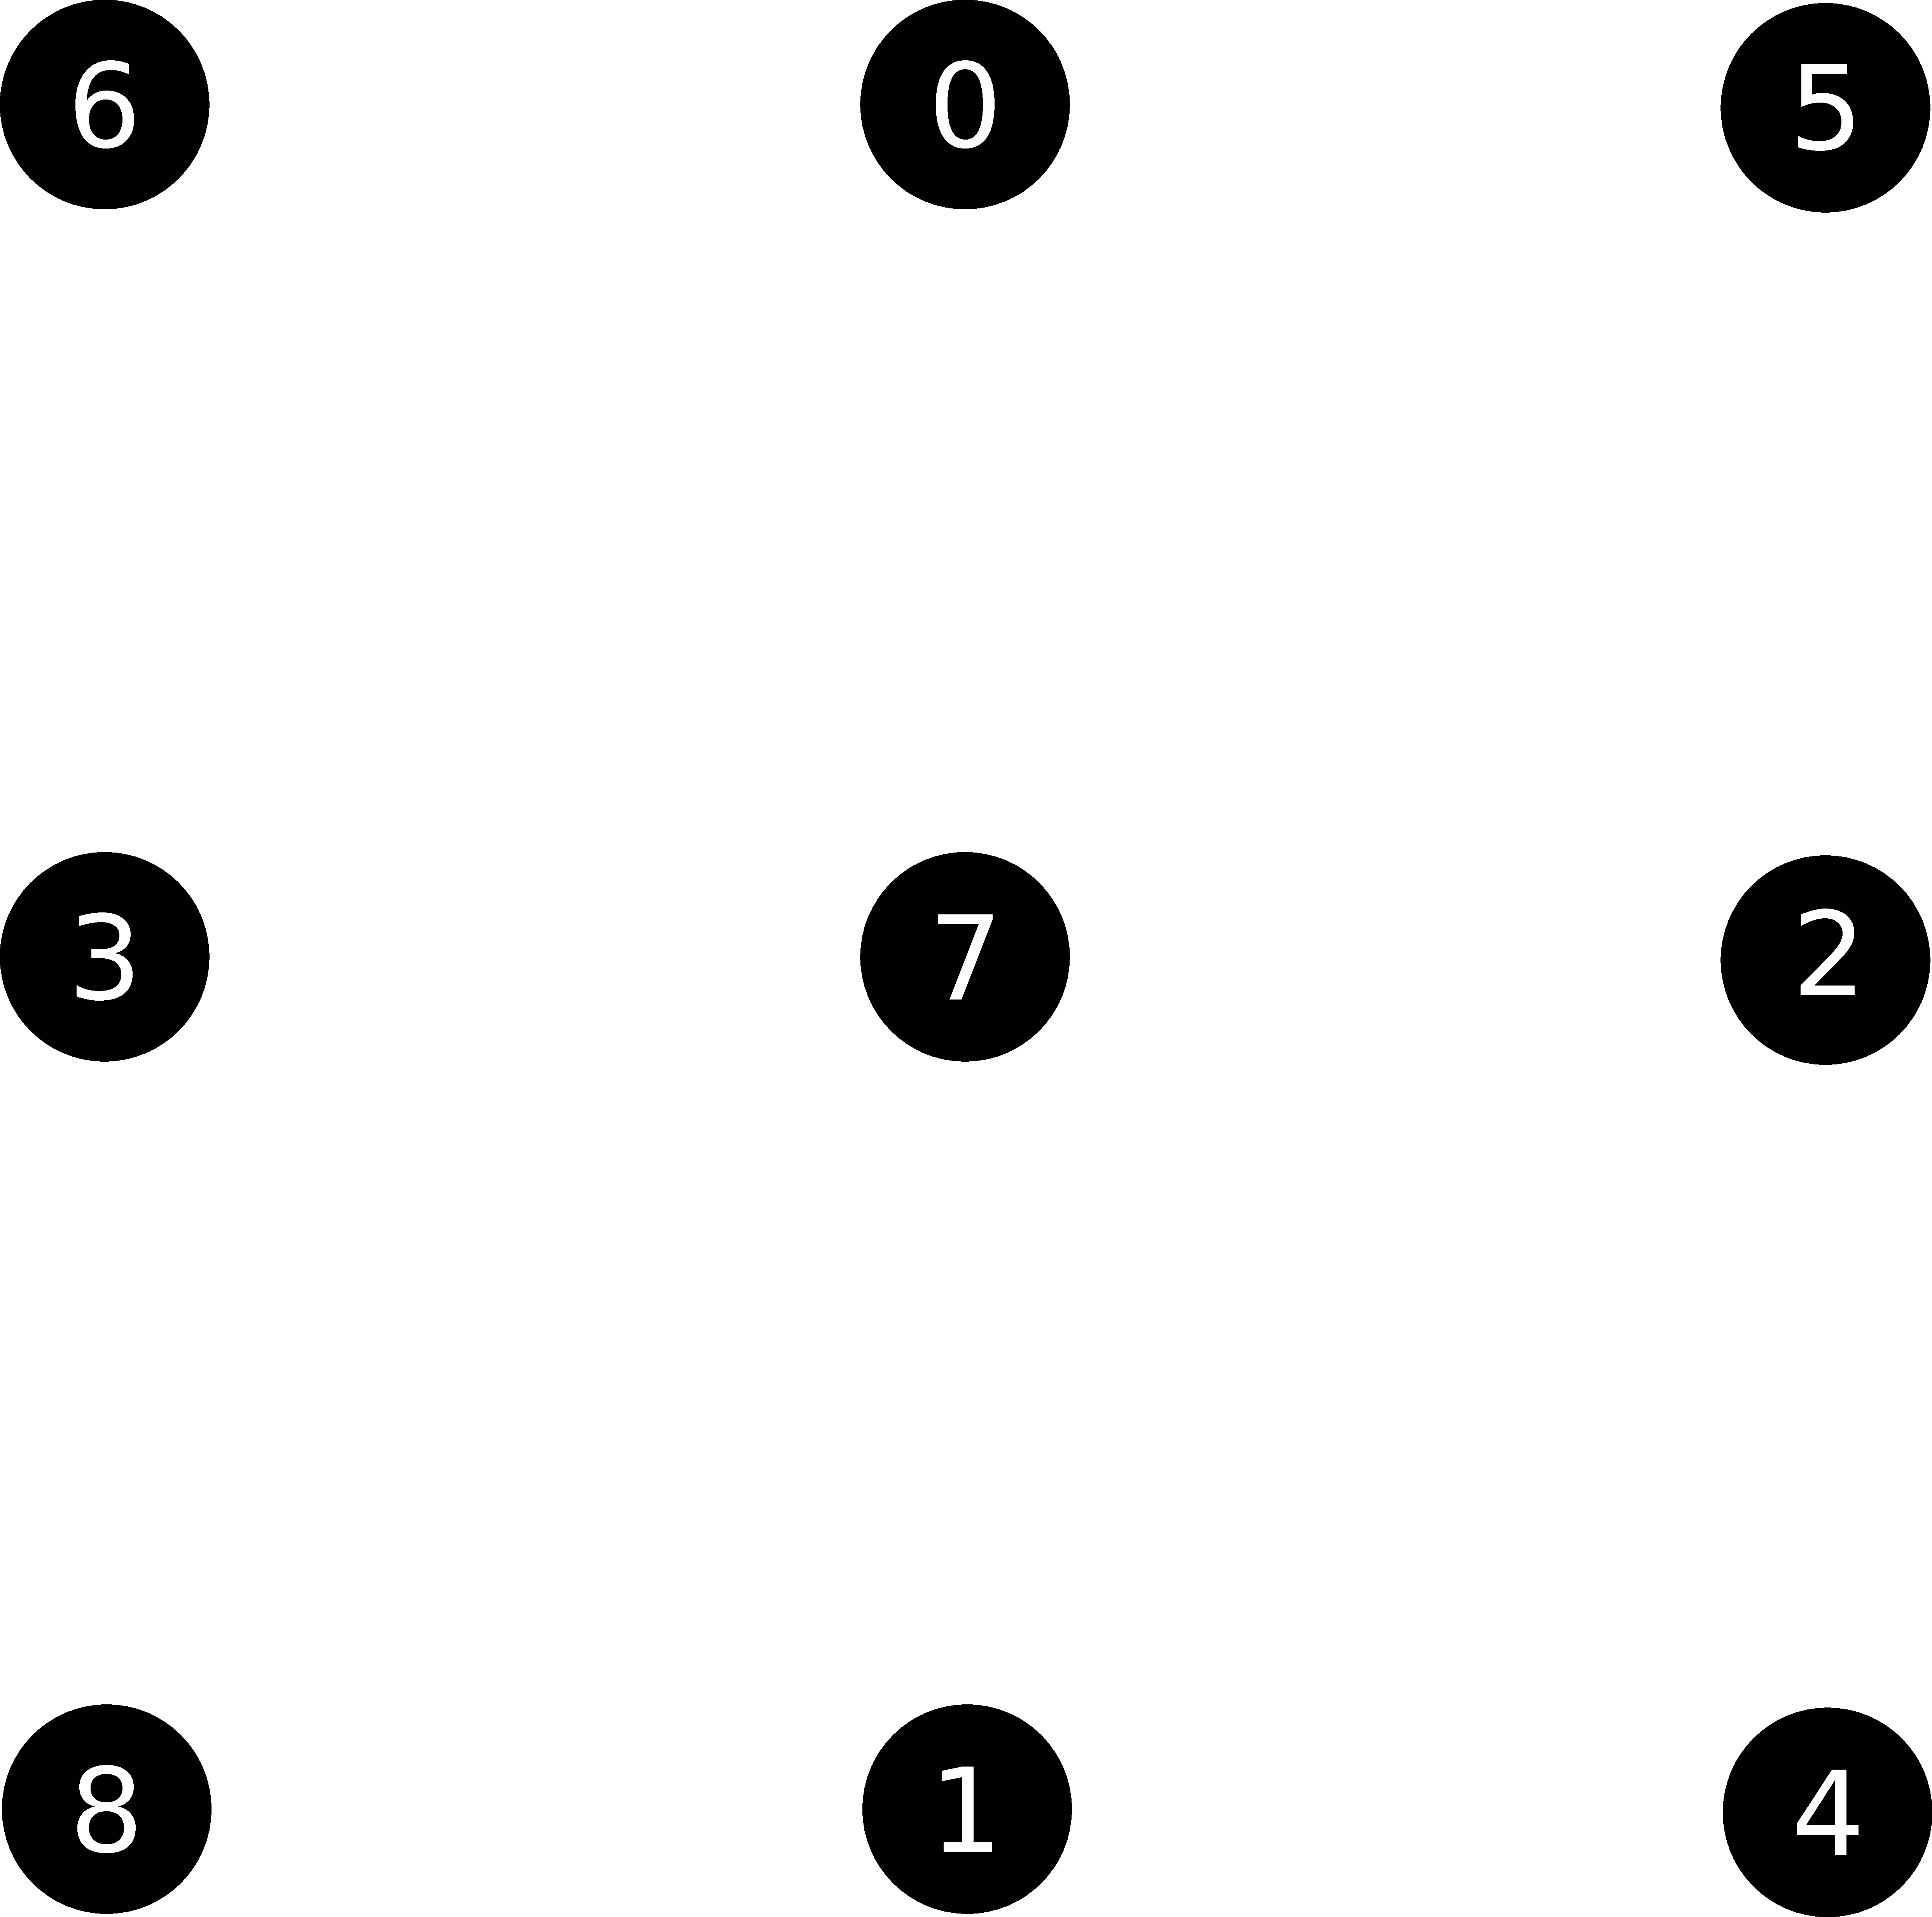
\includegraphics[scale=0.06]{./images/w3x3/w3x3-vertices.pdf}}}%
    \qquad \qquad \qquad
    \subfloat[Simplicial Mesh]{{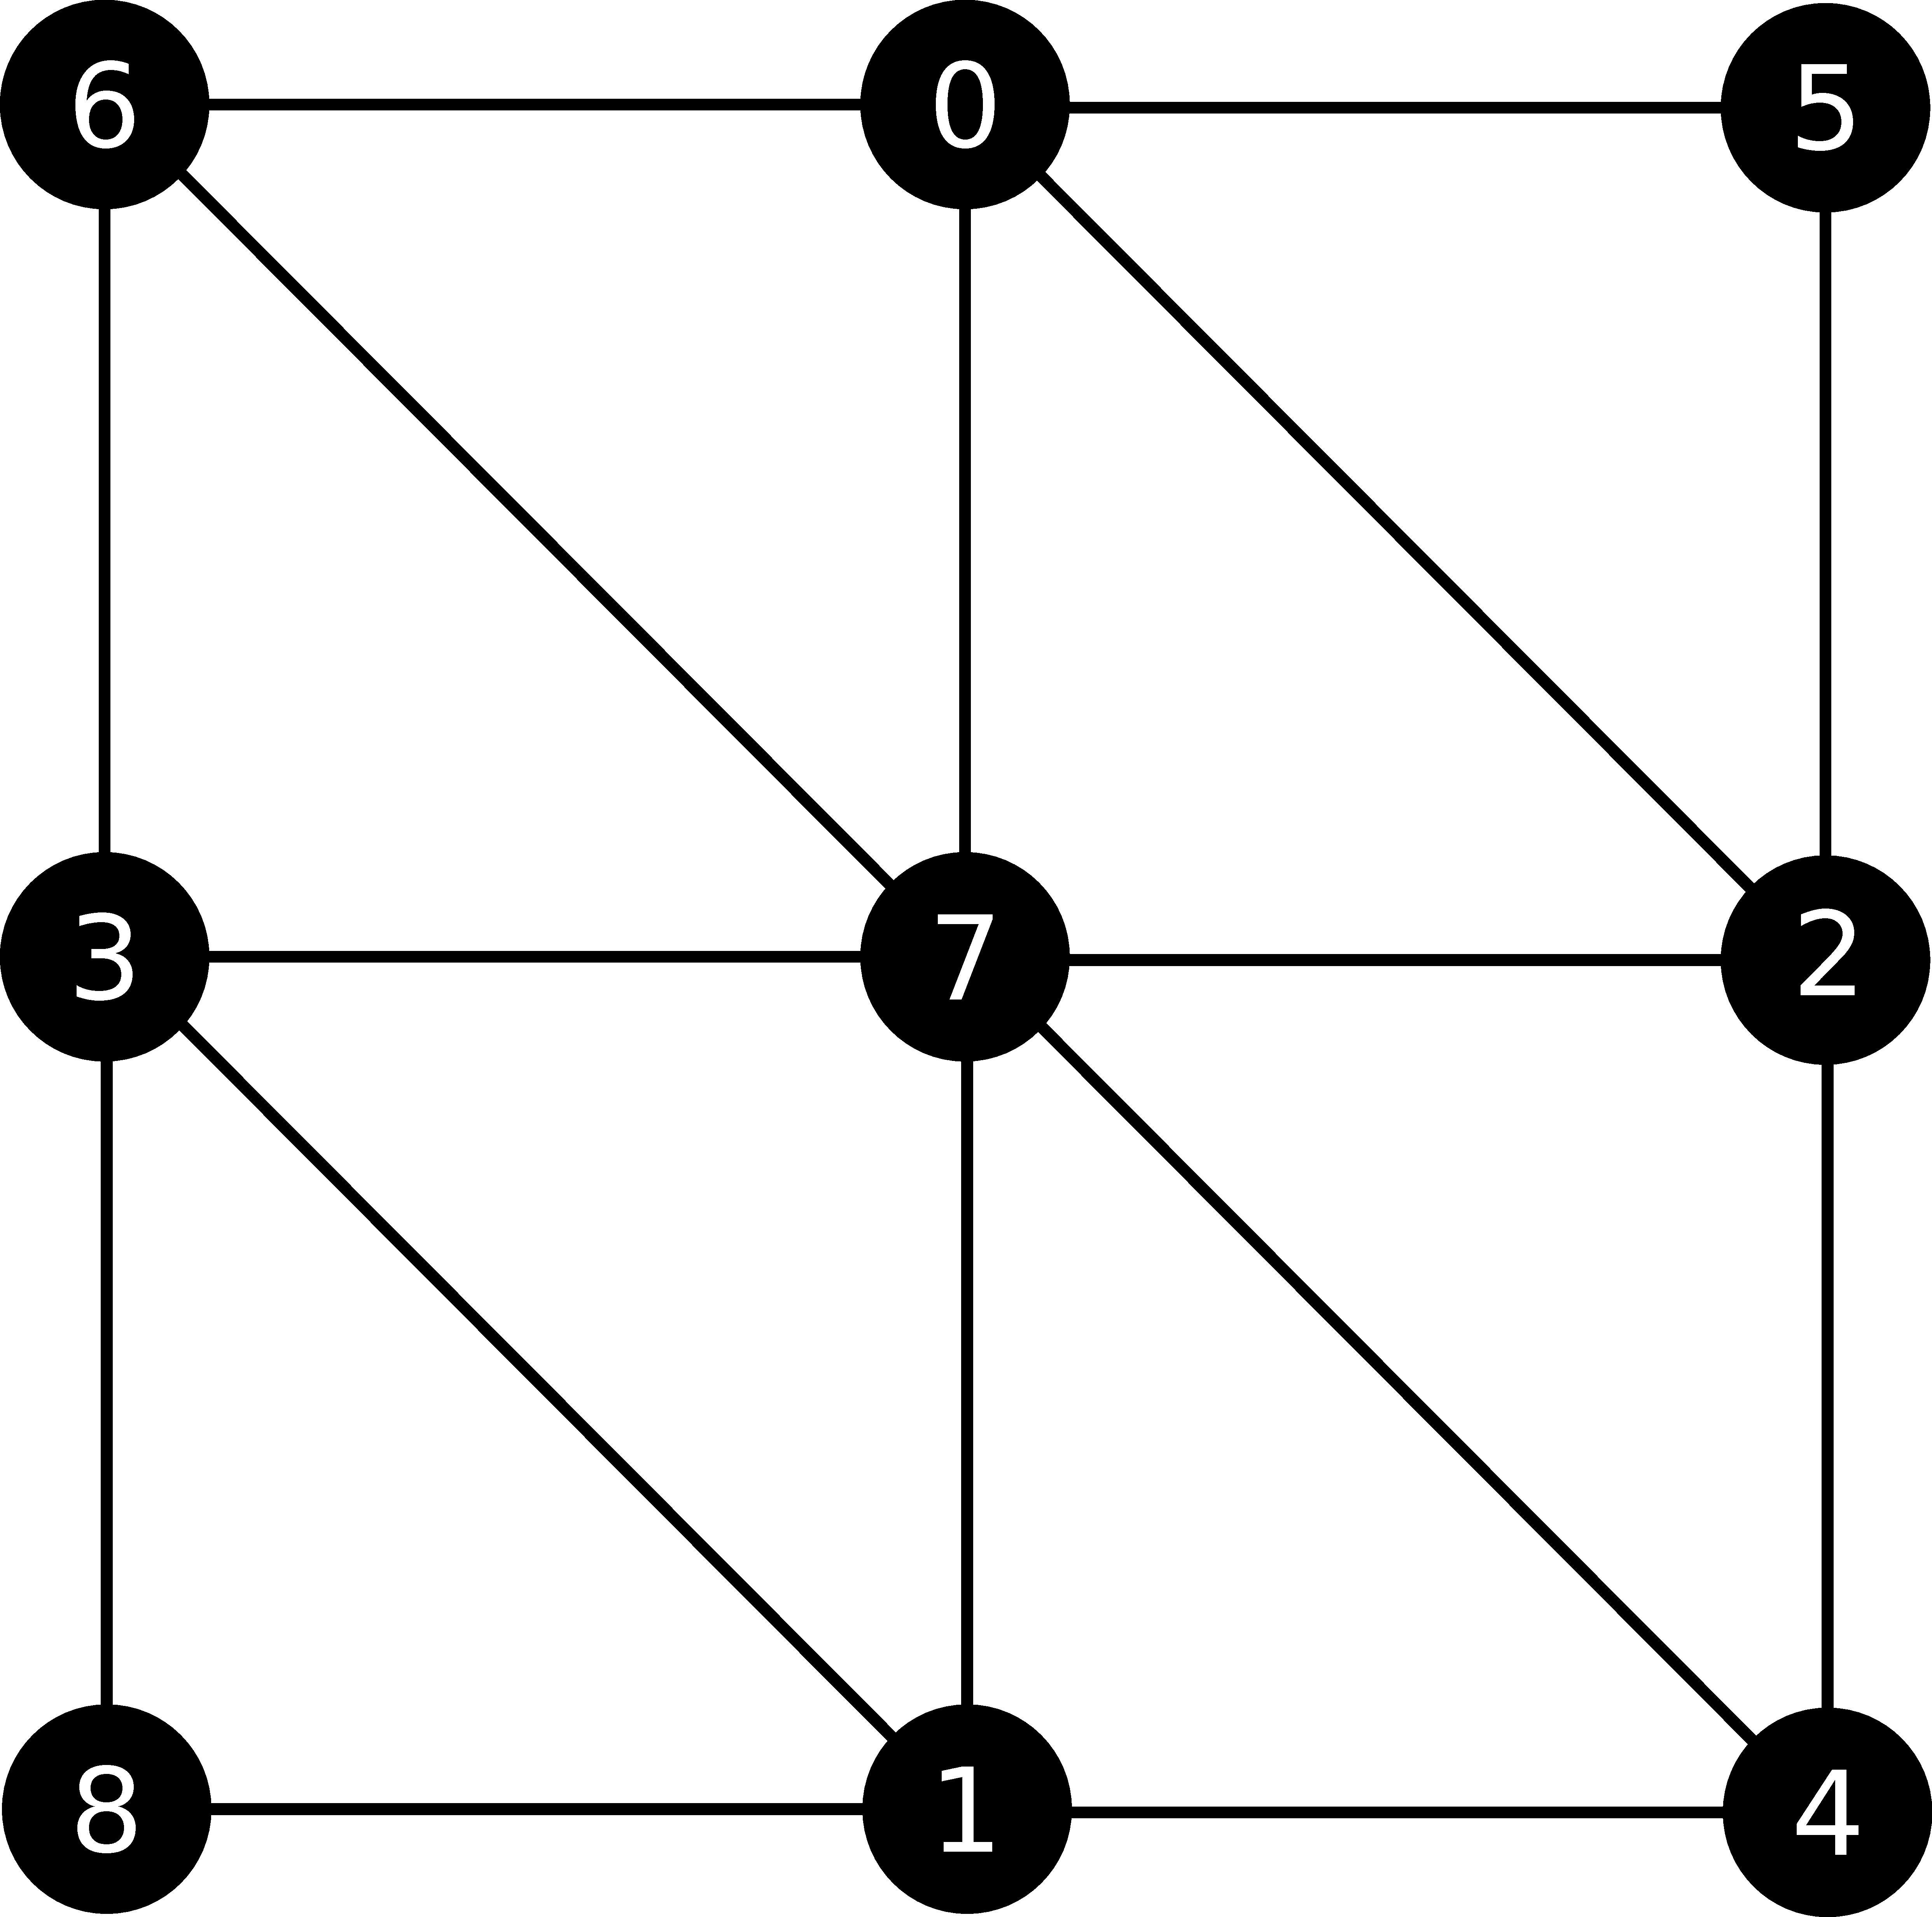
\includegraphics[scale=0.06]{./images/w3x3/w3x3-mesh.pdf}}}%
    \caption{Triangulation of input data to obtain a simplicial mesh.}%
    \label{fig:simplicial-mesh}%
\end{figure}
For simplicity and without loss of generality we will work with two-dimensional domains where the value samples are evenly spaced out in a grid-like fashion (Figure \ref{fig:simplicial-mesh}). The values of the approximation function at the simplicies are obtained via linear interpolation between the verticies of each simplex \cite{carr-masters}[]. As long as the original values we have sampled are unique it can be shown that the linear interpolation function is a Morse function and that all critical points are the vertices of the mesh \cite{curvature-embeded-polyhedra}.

\section{Contour Tree Computation}


 % @TODO What about higher dimensions and expand parallel stuff?

The first efficient algorithm for constructing contour trees \cite{first-ct-algo} is due to Van Kreveld et al. Its running time is $O(NlogN)$ on two dimensional domains and $O(N^2)$ in higher dimensions where $N$ is the number of triangles in the simplicial mesh. Tarasov and Vyalyi \cite{second-ct-algo} extended this algorithm to work in time $O(NlogN)$ on three dimensional domains. Their approach however involved a complicated procedure for dealing with multi-saddle points. Both algorithms suffer from lack of generality and non-trivial treatment of multi-saddle points. Carr at. al \cite{ct-big-paper} introduced an algorithm with running time $O(nlogn + N\alpha(N))$ where $n$ is the number of vertices in the simplicial mesh and $\alpha$ is the notoriously slow growing inverse Ackerman function. This algorithm works in any number of dimensions and has simple treatment of multi-saddle points.

More recent developments in the field focus on extending the existing algorithms to accomodate the distributed \cite{distributed-ct-algo, distributed-ct-algo-2} and shared memory parallelism paradigms \cite{parallel-peak-pruning, parallel-ct-1}. The focus of this dissertation we will be one of the latest devlopments in a data parallel shared memory algorithm for contour tree computation
\cite{parallel-peak-pruning}. Before introducing how that algorithm operates and one of the issues related to its parallel performance we will first give a more detailed overview of the most established serial algorithm \cite{ct-big-paper} on which the data parallel one is based on. In order to talk about any of the two algorithm we must establish some notation and define height graphs and trees as they are defined in \cite{carr-masters}.

% @TODO Finish this.
% Also define regular points!

\section{Height Trees}

% @TODO Talk about supernodes and superarcs

% @TODO Target application domain.
A height graph is a graph $G = (V, E)$ together with a real valued function $h$ defined on the vertices of $G$. Height graphs are also known in the literature as weighted graphs. We are changing our notation to be more indicative of the fact that the weight function is defined on the vertices and that it corresponds to height in our target application domain. A height tree is a height graph which is a tree. Contour trees are height trees because nodes in the contour tree correspond to nodes in the mesh and can inherit their height (sampled) value. Analogous to the assumption we have made about uniqueness of values we will also assume all vertices in the height trees we consider have unique heights. In other words $h(u) \ne h(v)$ for all $u ,v \in V(G)$ where $u \ne v$. The function $h$ naturally induces a total ordering on the vertices. From now on we will assume the vertices of $G$ are given in ascending order. That is to say, $V(G) = \{v_1, v_2, ... , v_n\}$ where $h(v_1) < h(v_2) < ... < h(v_n)$. This lets us work with the indices of the vertices without having to compare their heights directly. In this notation $h(v_i) < h(v_j)$ when $i < j$.

%@TODO Remove this if you will not use it.

Introducing the height function allows us to talk about ascending and descending paths. A path in a graph is a sequence of vertices $(u_1, u_2, ... , u_k)$ where $u_i \in V(G)$ for $i \in \{1, 2, ..., k\}$ and $u_iu_{i+1} \in E(G)$ for $i \in \{1, 2, ..., k-1\}$. A path in a height graph is ascending whenever $h(u_1) < h(u_2) < ... < h(u_k)$. If we traverse the path in the opposite direction it would be descending. We will simply call these paths monotone whenever we wish to avoid committing to a specific direction of travel.

When working with height graphs it is useful to extend the definition of a degree of a vertex by taking the height function into account.

\begin{defn} Let $G$ be a height graph and $v$ a vertex of $G$. The up degree of $v$ is defined as the number of neighbours of $v$ with higher value. It is denoted as $\delta^+(v) = \big|\{ u \in N(v) : h(u) > h(v) \}\big|$.   \end{defn}

The down degree of a vertex $v$ is defined analogously as $\delta^-(v) = \big|\{ u \in N(v) : h(u) < h(v) \}\big|$. In the context of height trees the definitions of up and down degrees of a vertex allow us distinguish between two types of leafs - lower and upper leafs.
\begin{defn} Let $G$ be a height graph and $v$ a vertex of $G$. If  $\delta^+(v) = 1$ and $\delta^-(v) = 0$ then $v$ is a lower leaf.  \end{defn}

If $\delta^+(v) = 0$ and $\delta^-(v) = 1$ then $v$ is an upper leaf. We will see in the next section how differentiating between the two types of leafs is a crutial part in the computation of the contour tree.

\section{Serial Algorithm}

The contour tree is a tree that consists of []:

\begin{itemize}
    \item Vertices or supernodes that correspond to level sets that contain a critical point.
    \item Edges or superarcs correspond to path-connected regions bounded by two level sets which both contain a critical point. They connect the supernodes those level sets correspond to.
\end{itemize}

% @TODO Think about this contruction and destruction business
The contour tree contains information of four types of events - creation, destruction, joining and splitting of contours. We can derive from the contour tree two other height trees that each contain the information of cretion and joining and destruction and splitting separately. We will call these the join and split trees. The join tree contains information for the contours that are created and joined together and the split tree holds the information for the contours that are destroyed or that split apart. The join tree of a contour tree summarises the evolution of the connectivity of the sublevel sets of the interpolation function and the split tree of the superlevel sets. You can find an example of the join and split trees of Figure \ref{fig:mesh-join-split-contour}.

% The two are symmetric in that the join tree of the function $f$ is isomorphic to the split tree of the negative of the function $-f$.

\begin{figure}[h]%
    \centering
    \subfloat[Simplicial Mesh]{{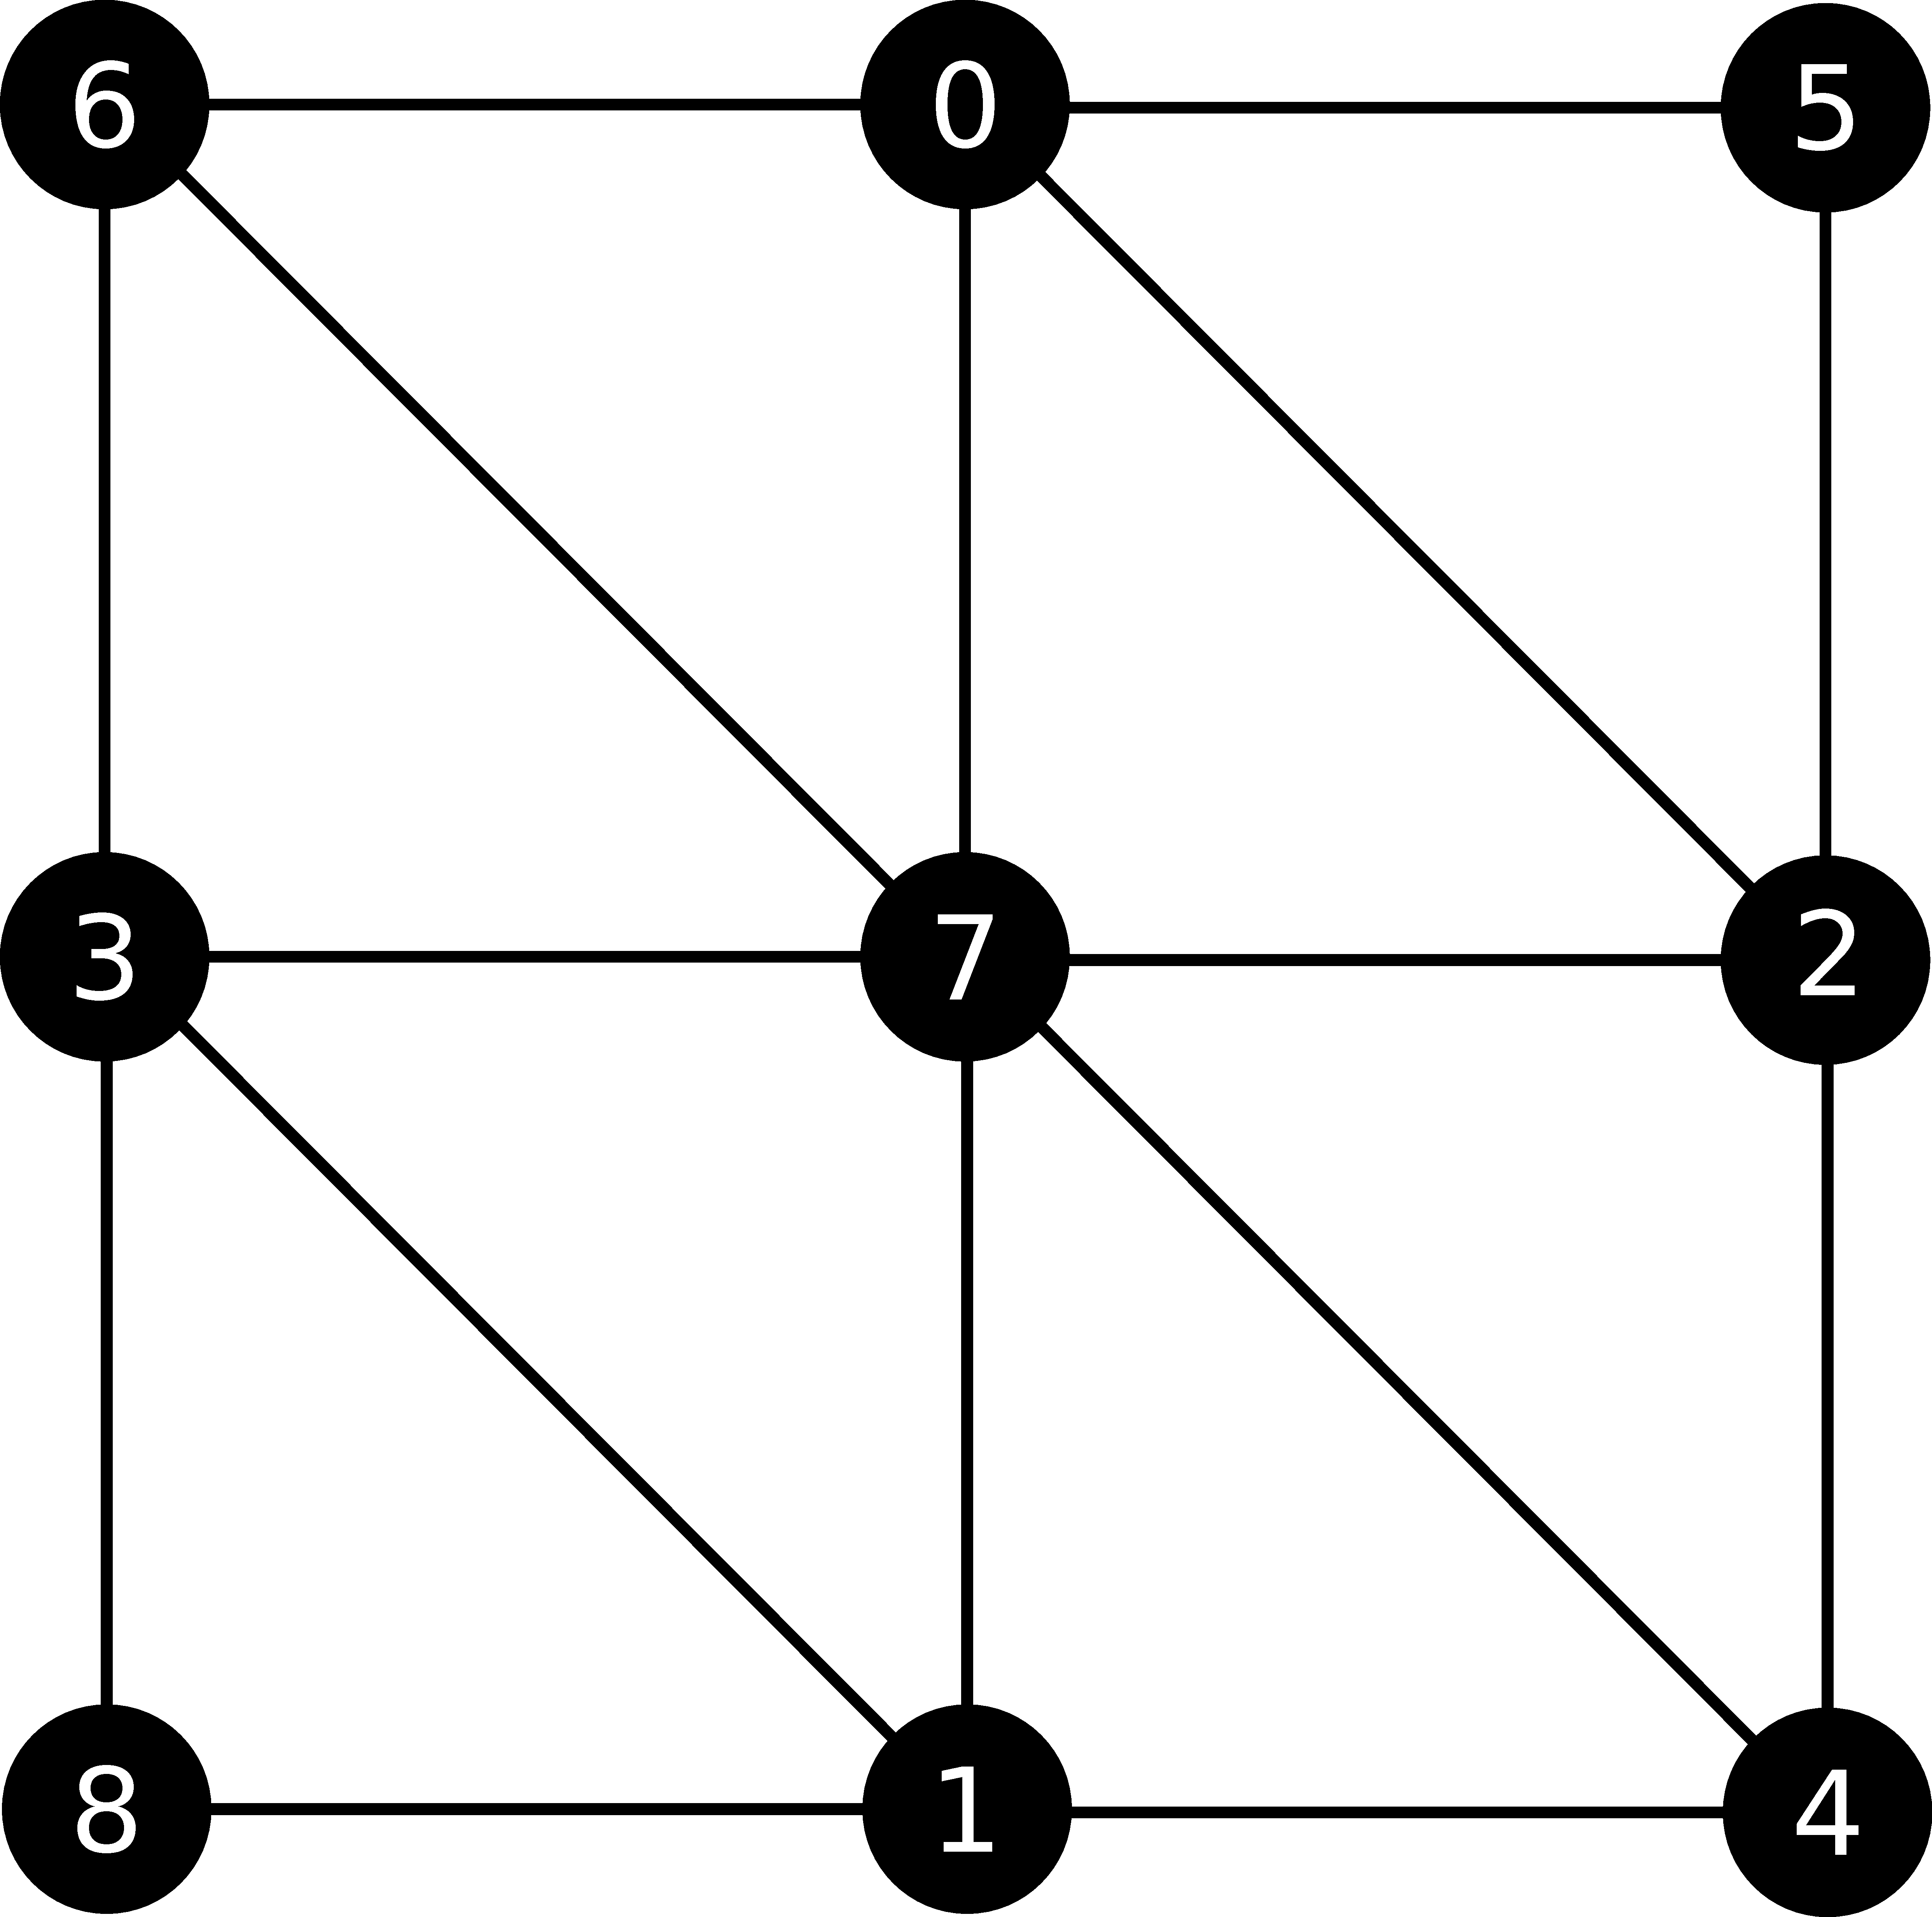
\includegraphics[scale=0.06]{./images/filtration/asc/x9.pdf}}}%
    \qquad \qquad \qquad
    \subfloat[Contour Tree]{{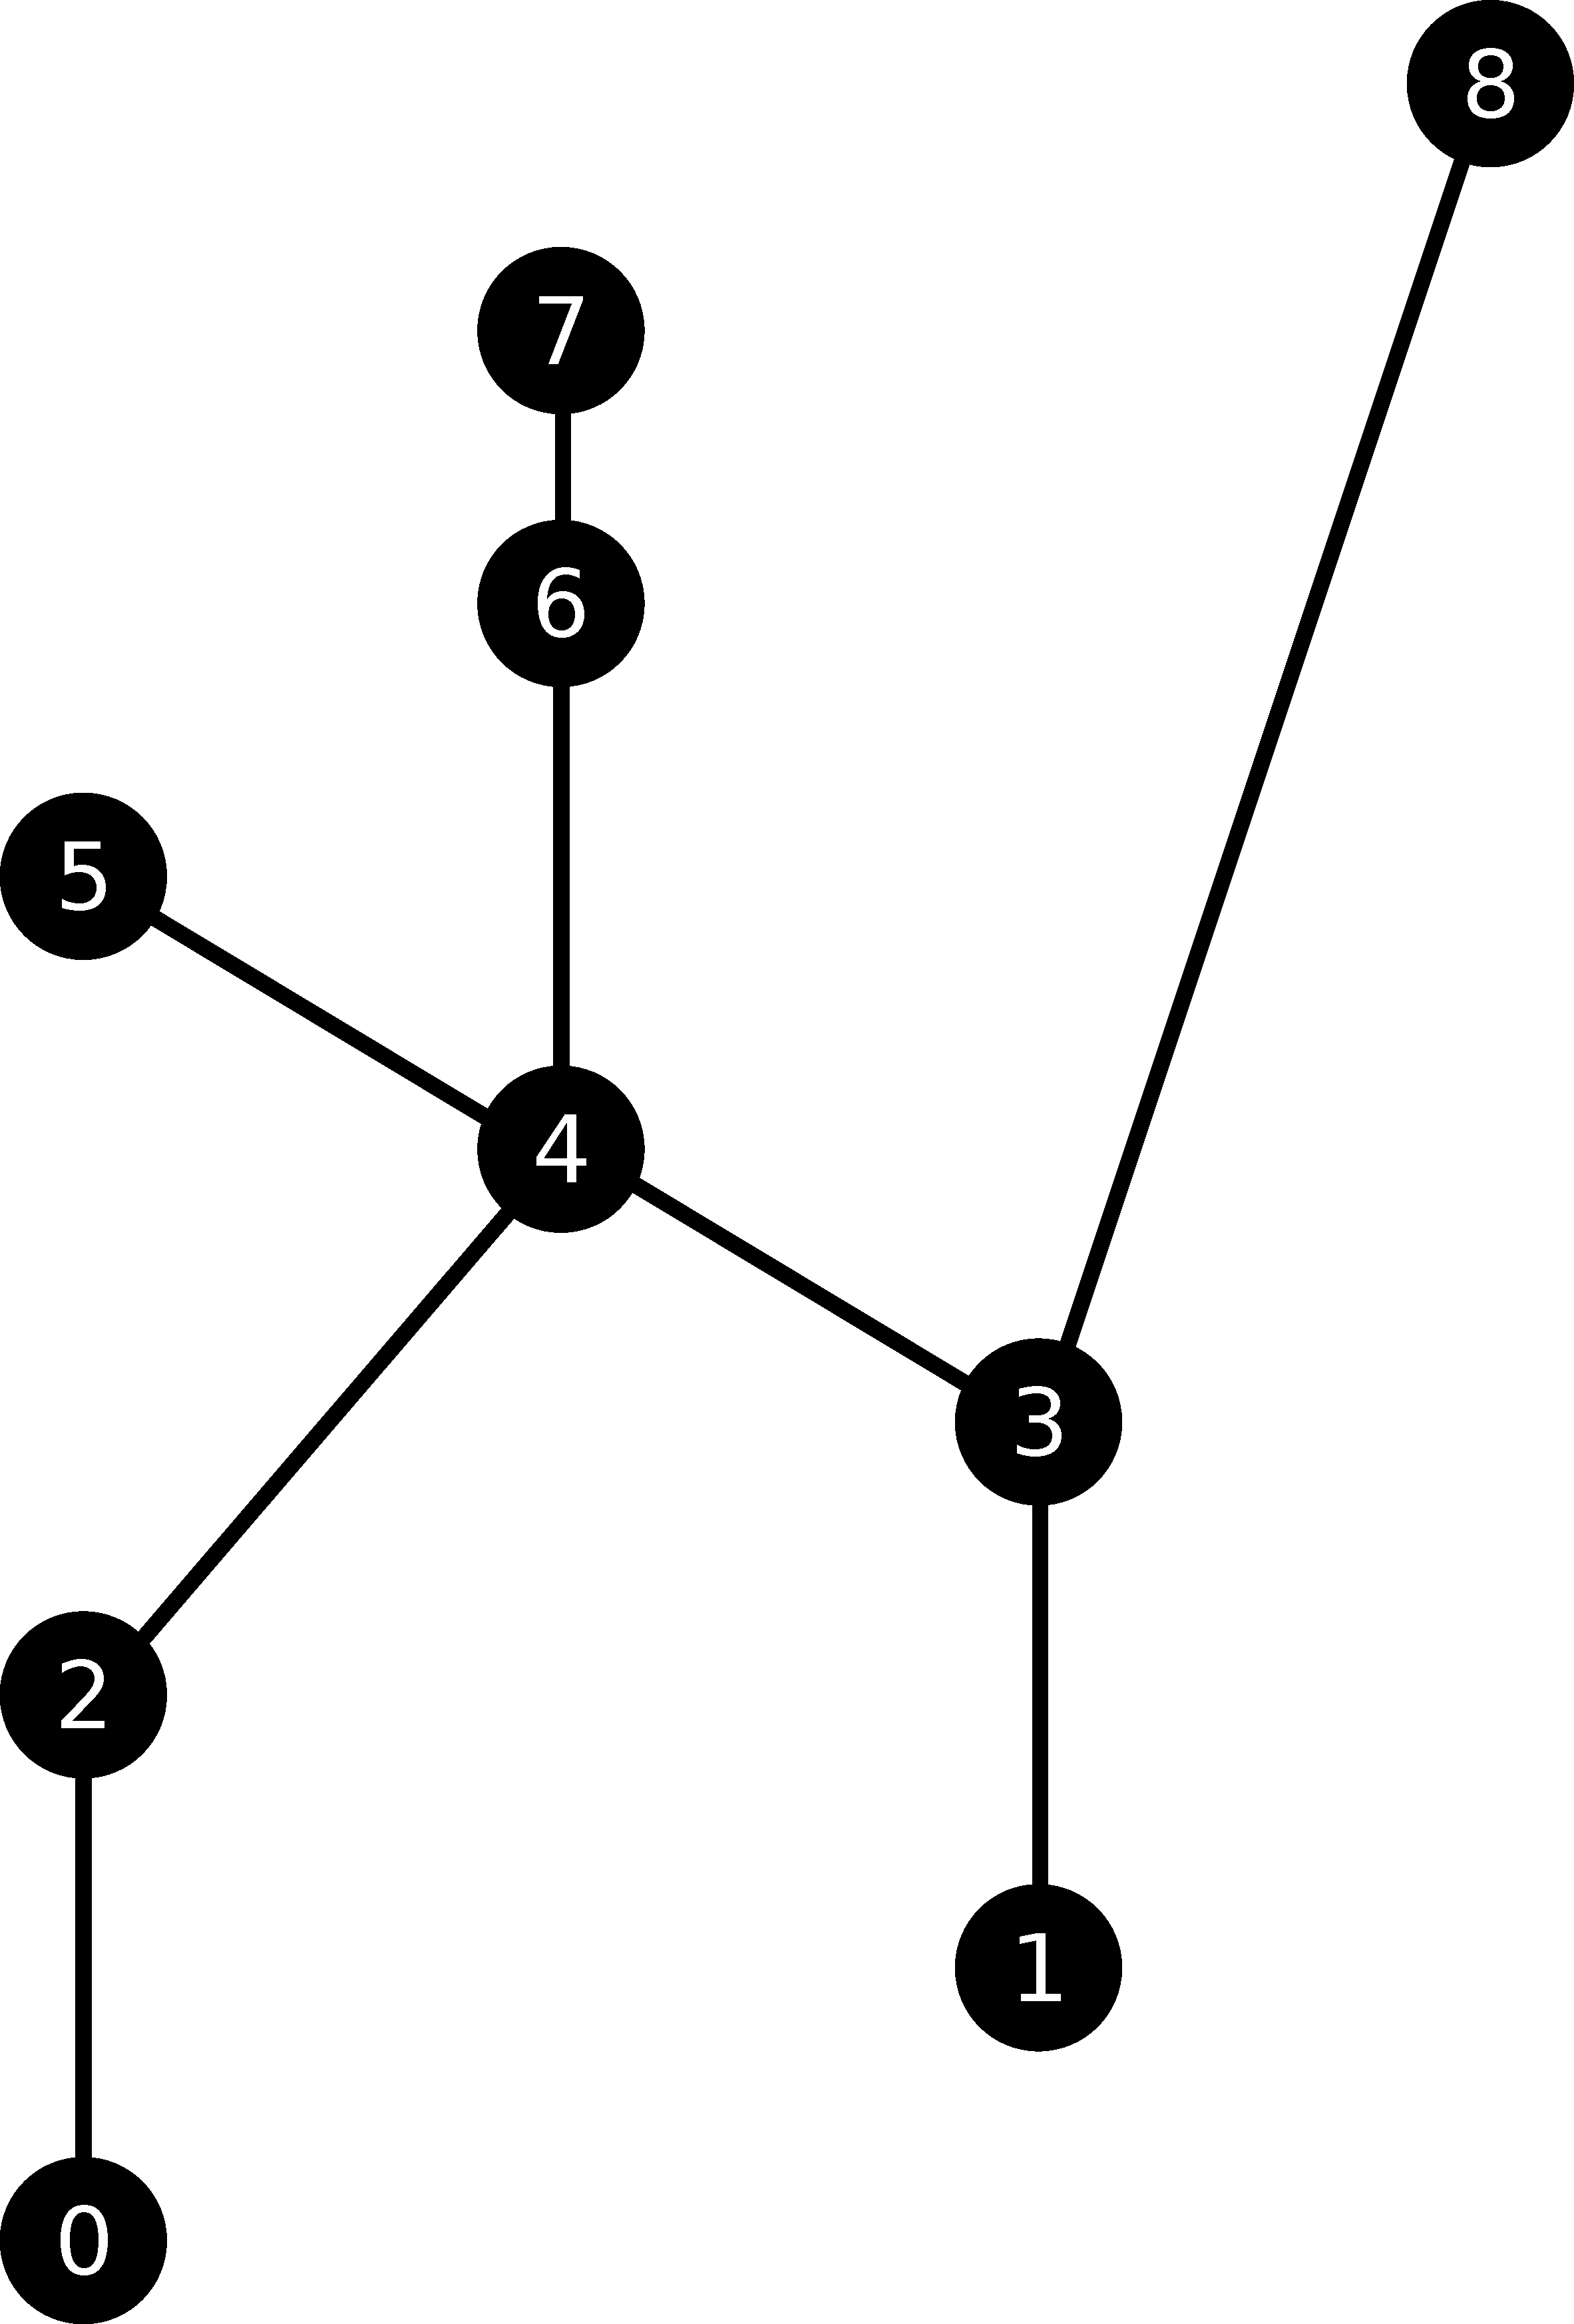
\includegraphics[scale=0.10]{./images/w3x3/w3x3-contour-tree.pdf}}}%
    \qquad \qquad \qquad

    \subfloat[Join Tree]{{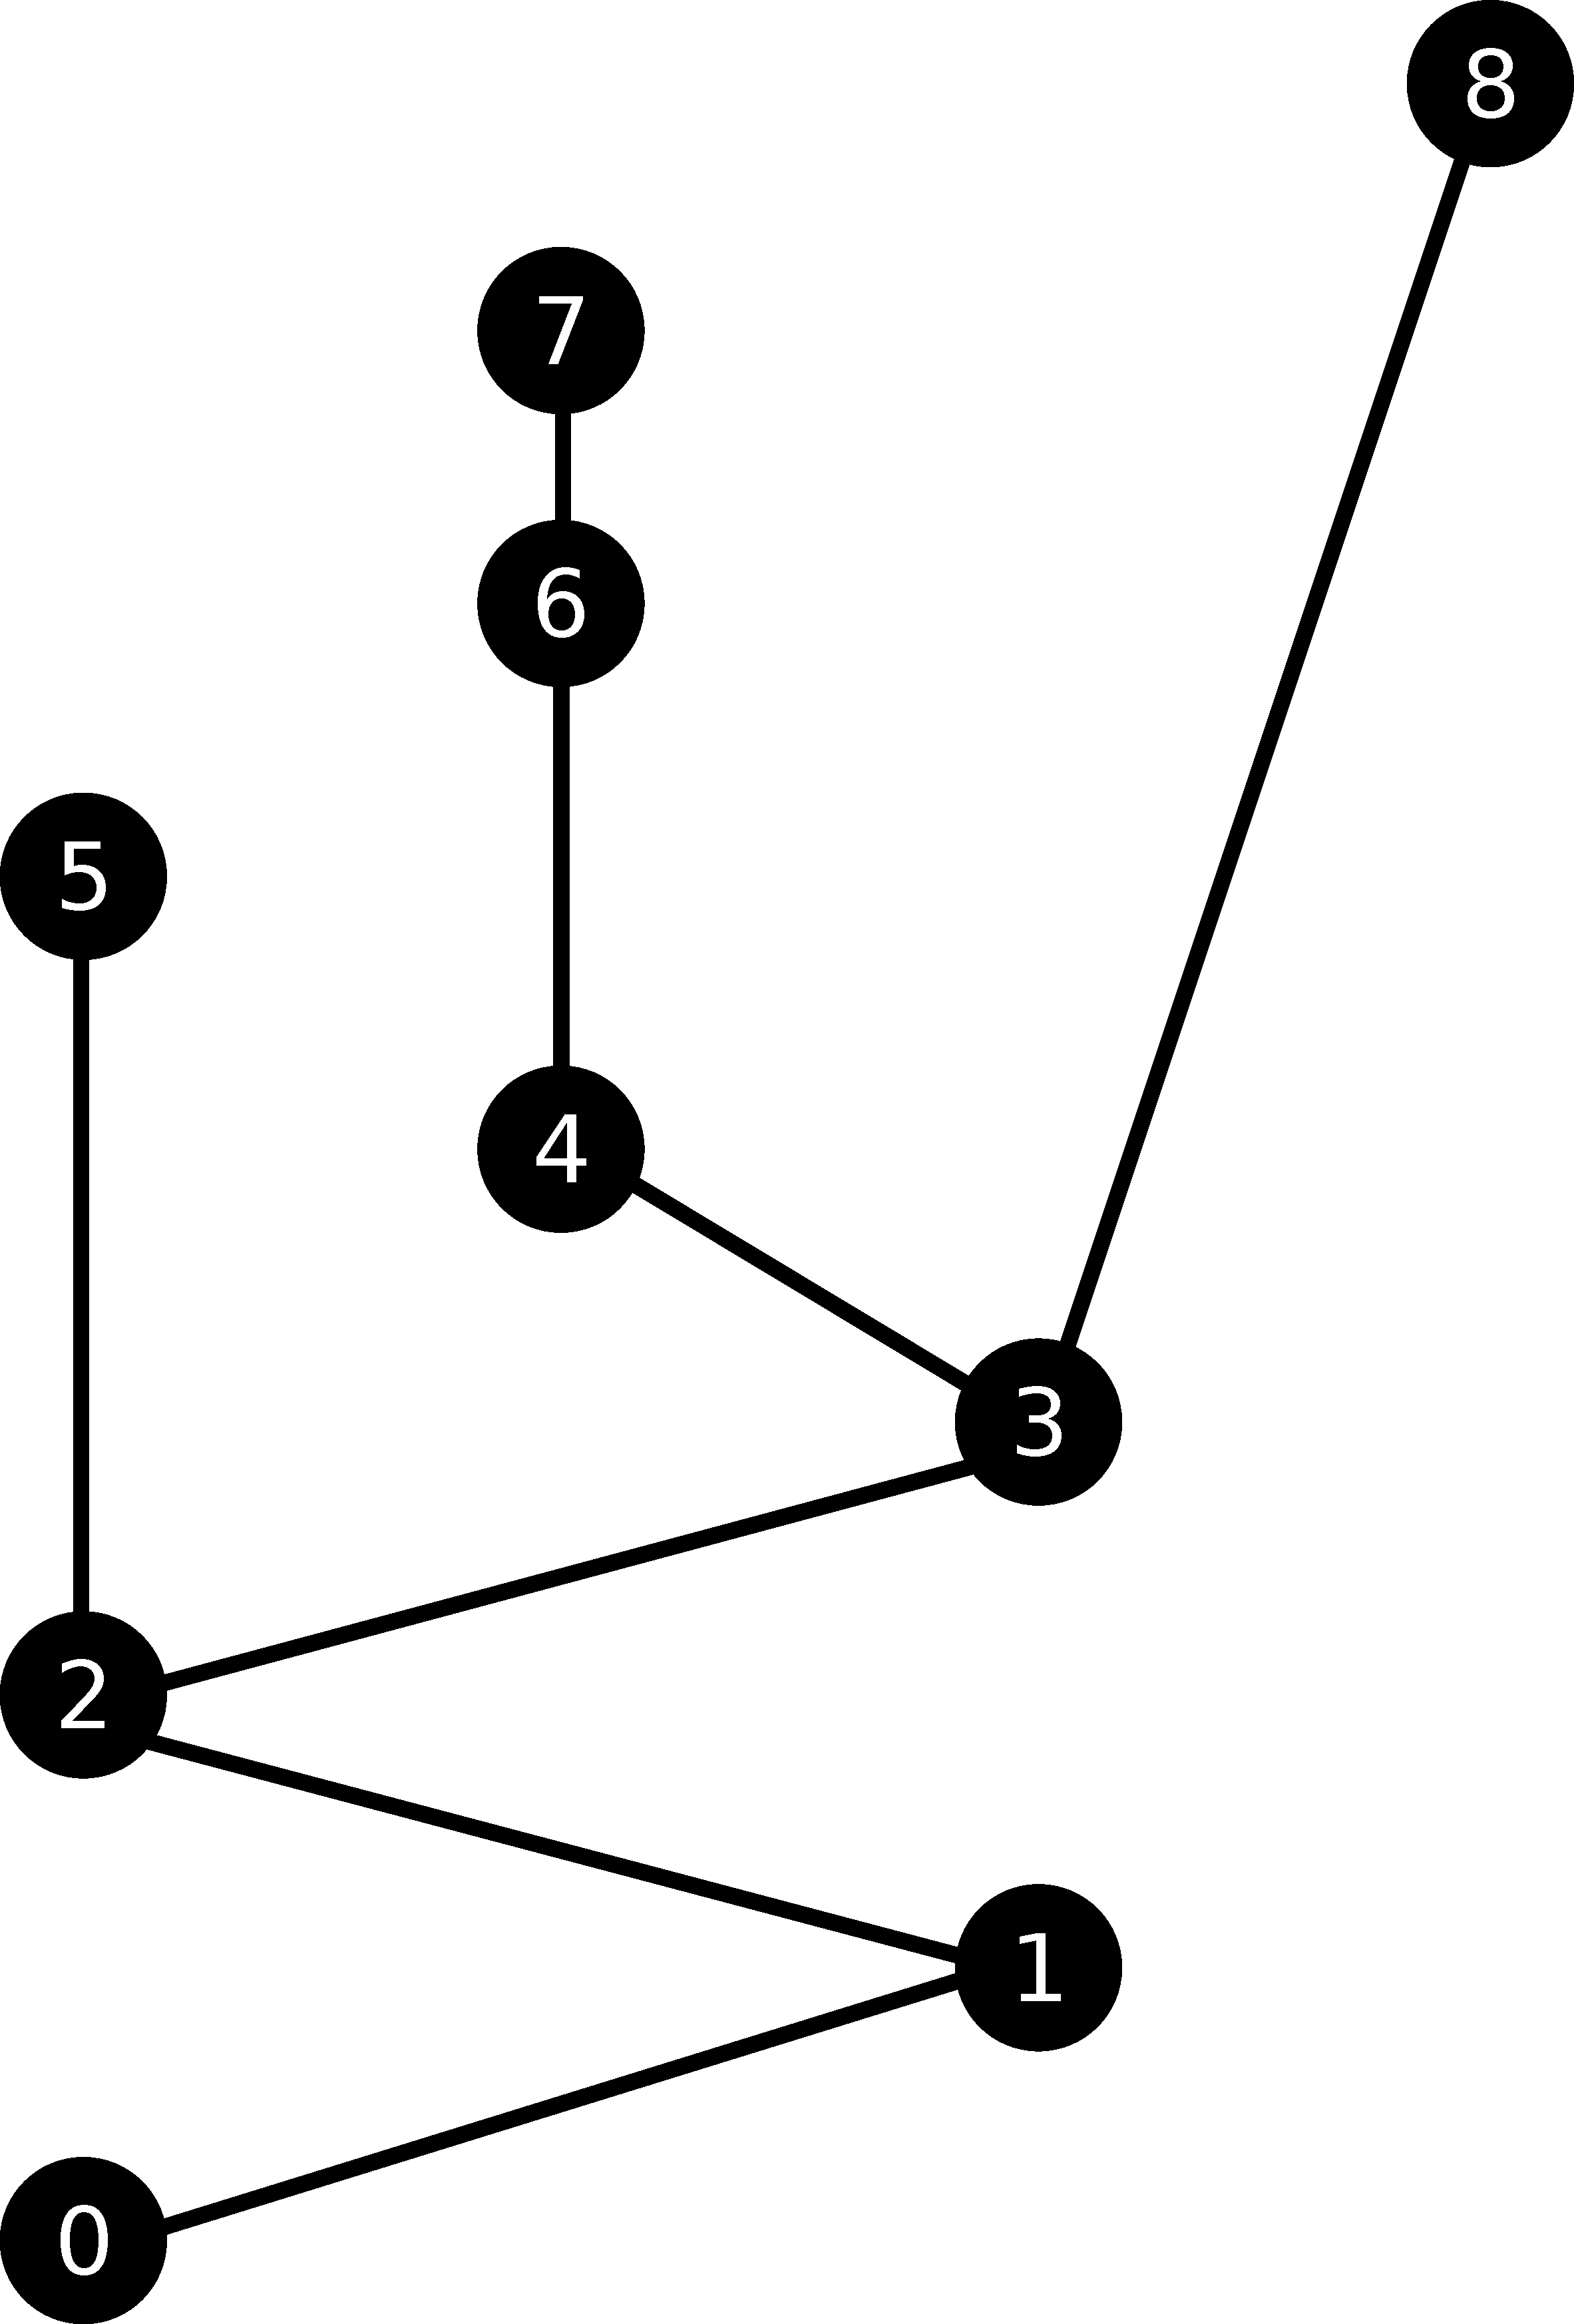
\includegraphics[scale=0.10]{./images/w3x3/w3x3-join-tree.pdf}}}%
    \qquad \qquad \qquad
    \subfloat[Split Tree]{{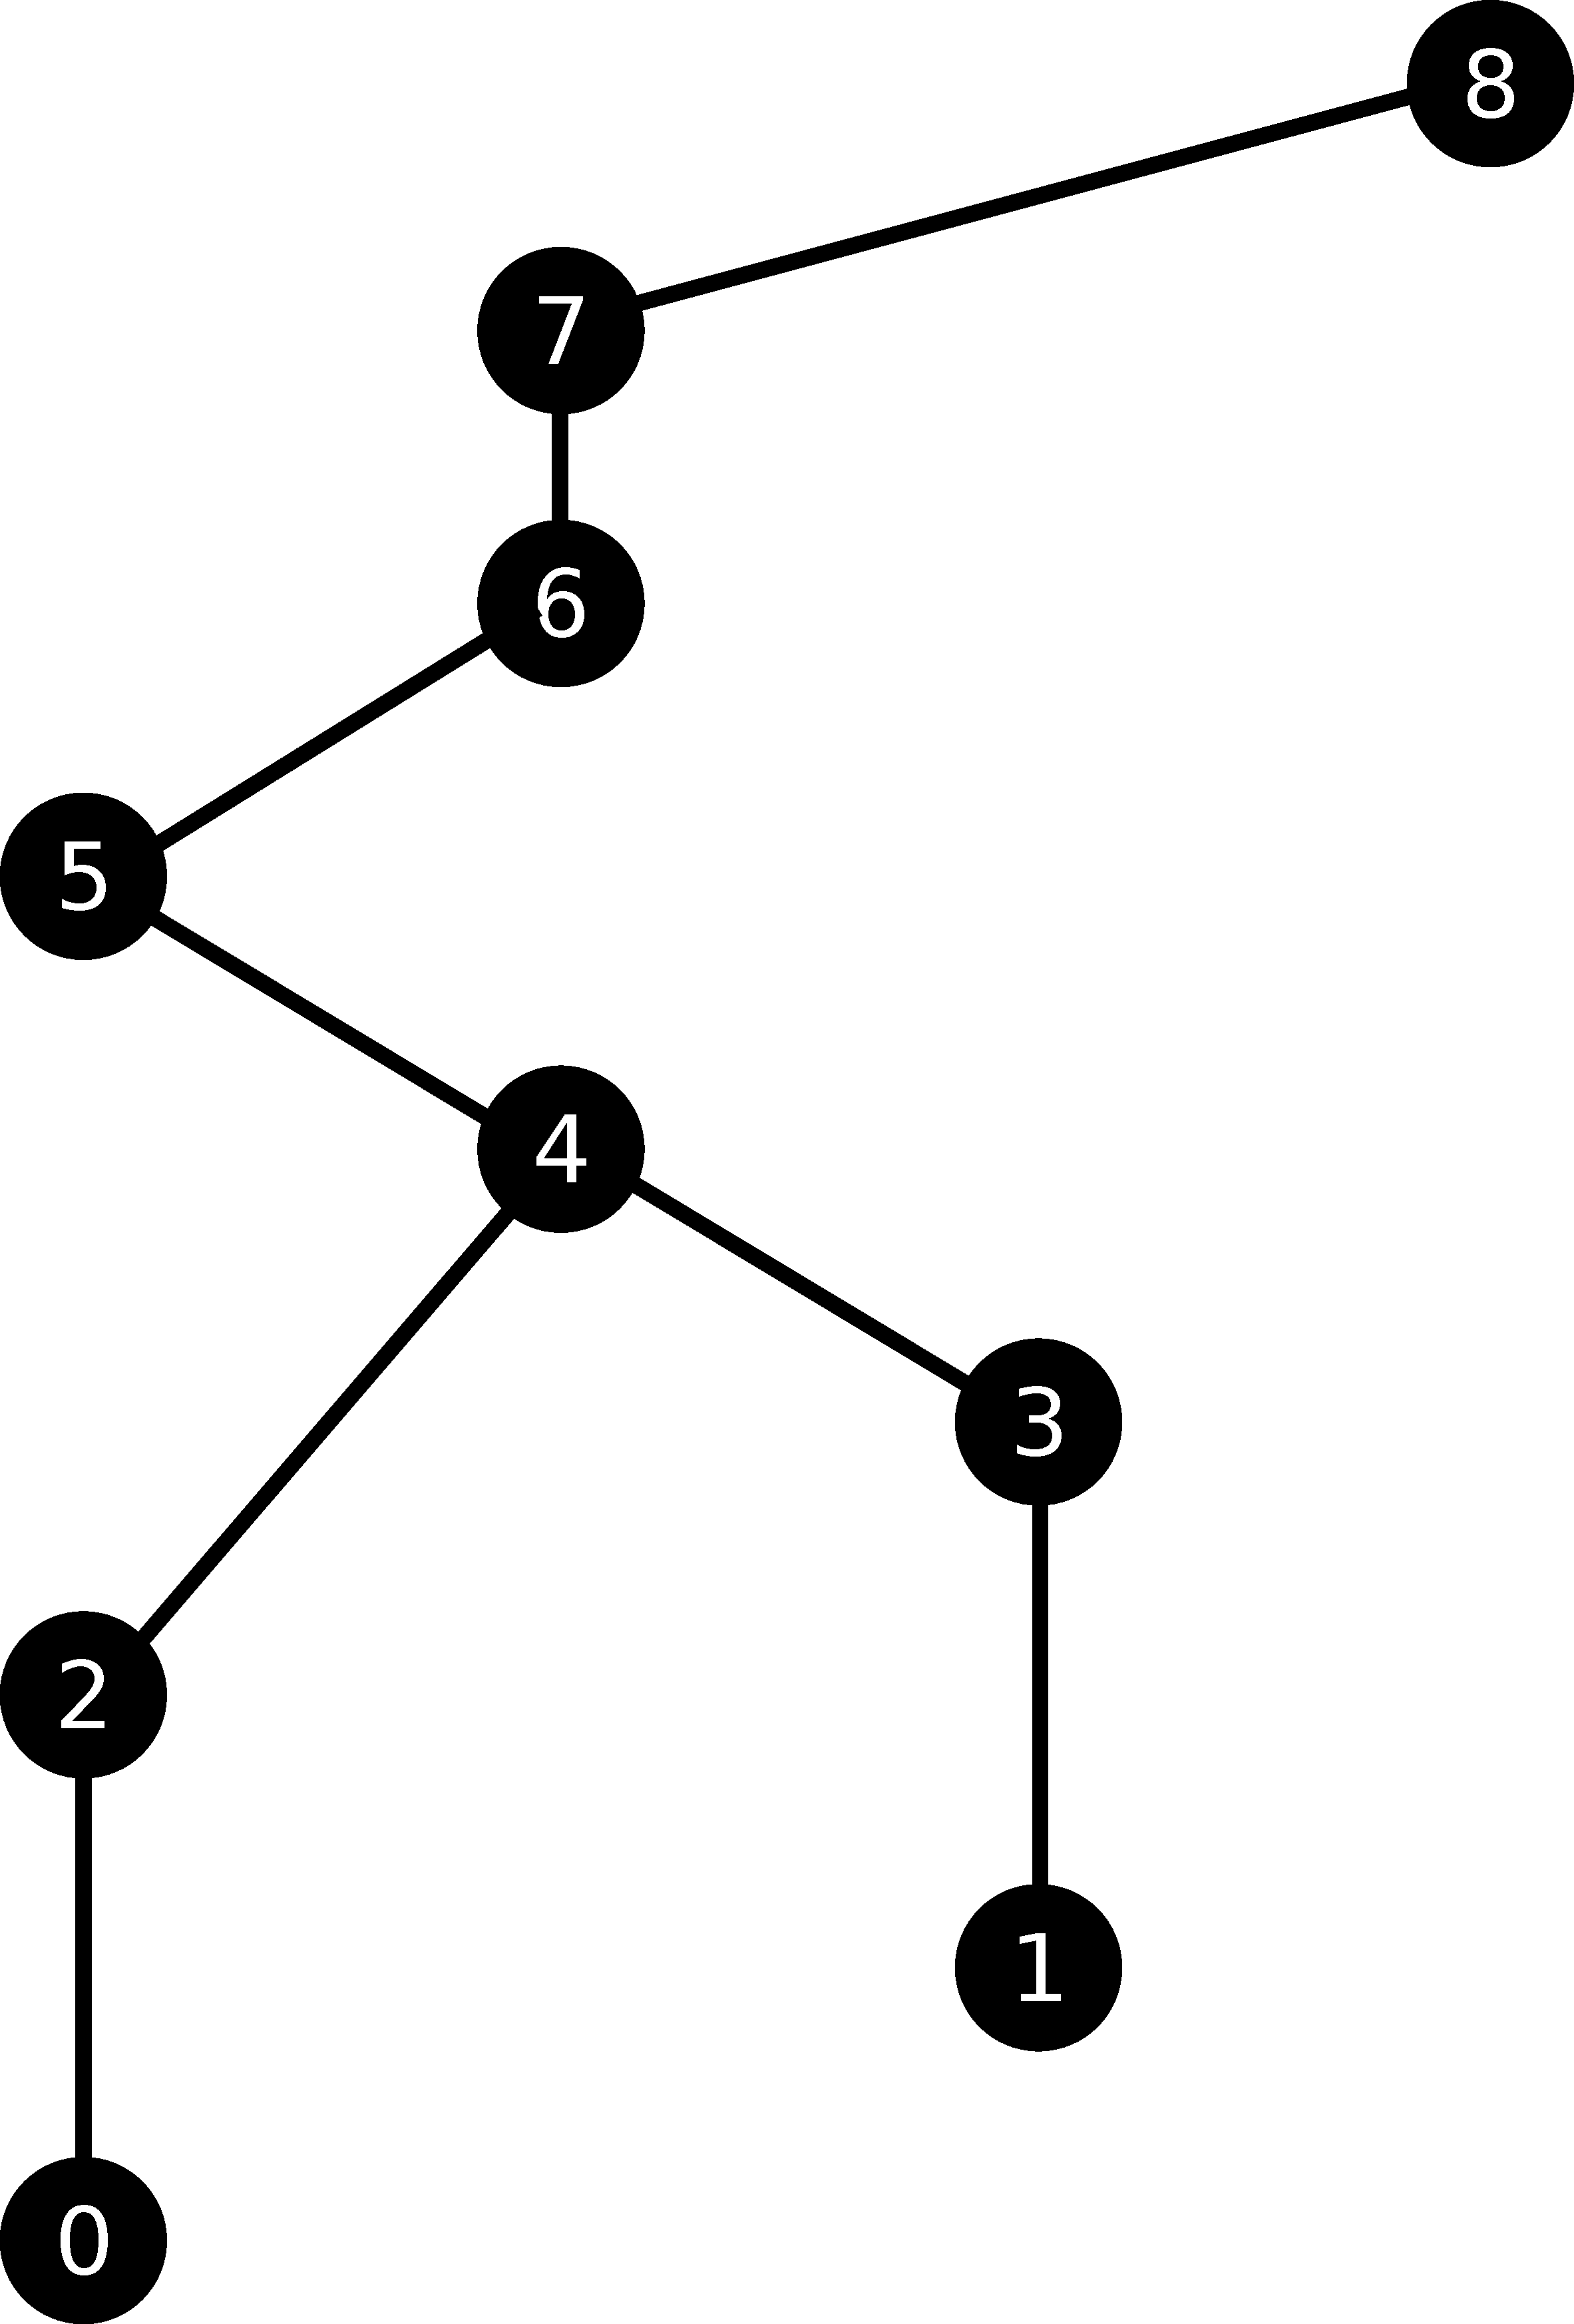
\includegraphics[scale=0.10]{./images/w3x3/w3x3-split-tree.pdf}}}%
    \caption{The Simplicial Mesh, Join and Split Trees and Contour Tree.}%
    \label{fig:mesh-join-split-contour}%
\end{figure}

The reason we would like to study join and split trees is that the contour tree can be reconstructed from them. The core idea of the algorithm we will present is that we can derive the join and split trees directly from the simplicial mesh and then combine them to obtain the contour tree. We will first describe how the join and split trees are computed from the mesh. We only have to describe the process for the join tree because their construction is symetrical [].

\begin{defn} A join component is a connected component in the superlevel set $f^{-1}([h, \infty))$ at some $h \in \mathbb{R}$.  \end{defn}

Let $M$ be the simplicial mesh from Figure \ref{fig:mesh-join-split-contour} (a) and let $h : M \to \mathbb{R}$ be the interpolation function defined on it. We will refer to $h$ as the height function. To construct the join tree we are going to have to keep track of which components merge together in the superlevel sets of $h$. We will consider all superlevel sets $M^t = h^{-1}([t, \infty)) = \{x \in M : h(x) \in [t, \infty) \}$ as a one parameter family $\{M^t\}_{t \in \mathbb{R}}$
of nested subsets of $M$. We can see from this definition that $M^a \subseteq M^b$ whenever $a \le b$. What the join tree captures is how the connectivity of the superlevel sets changes as the parameter $t$ is increased. The connectivity of superlevel sets changes either at local minima where a new component is created or a saddle point that merges two or more join components.

%We will not formalise the notion of tracking join components and constructing a join tree. Let us work in the general setting where $X$ is any path-connected topological space and $h : X \to \mathbb{R}$ is a function defined on $X$. The claims we make will hold in the special case where $X$ is a simplicial complex. Let us consider all sublevel sets $X_t = h^{-1}((-\infty, t]) = \{x \in X : h(x) \in (-\infty, t] \}$. They form a one parameter family $\{X_t\}_{t \in \mathbb{R}}$ of nested subsets where $X_a \subseteq X_b$ whenever $a \le b$. What the join tree captures is how the connectivity of the sublevel sets changes as the parameter $t$ is increased.

To visualise this process we can contract every join component to a point much like we did in the Reeb graph. The only difference here is that the equivalence relation is defined for all points in a superlevel set $h^{-1}([t, \infty))$ instead of a level set $h^{-1}(\{t\})$. Because of this change and because join components can only merge the join tree is a tree \cite{comp-topo}. Furthermore if $M_m = M$ is the last superlevel set for some $m \in \mathbb{R}$ then all join components merge into one because $M$ is path connected.

% @TODO Add citation

We will briefly outline the algorithm for constructing the join tree and refer the reader to \cite{ct-big-paper} for further implementational details. We know that all crical points are vertices of $M$ and that it is only at the critical points that changes in the topology of the superlevel sets can happen. The algorithm works by considering the vertices of the simplicial mesh in ascending order of their height. If the current vertex is a local minimum we directly add it in the join tree because it starts a join component. If the current vertex is a saddle that joins two or more components (join saddle) we add it to the join tree and add an edge between it and the local minima of the join components it merges. At the end of the computation all vertices will be in the same join component. In order to keep track of which join components different vertices belong to we can use the union-find data structure. The term  $\alpha(n)$ in the time complexity of the contour tree algorithm come from the basic operations of find and search in the union-find data structure.

% @TODO Define Join Saddles and Subdivided edges
Not all vertices of the mesh will be in the join tree. Only those which correspond to local maxima and to join saddles. This will pose a problem later on when we wish to combine the join and split trees. To avoid this problem we can augment the join tree by adding all missing vertices. This is done through edge subdivision. Let $a \text{ and } b$ be two adjacent vertices in the join tree.  Let $\{v_1, v_2, ..., v_n\}$ be vertices in the mesh that are not in the join tree that are given in ascending order in terms of height.  Suppose that $h(a) < h(v_i) < h(b)$ for all $i \in \{1, 2, ..., n\}$ and the vertices $v_i$ are in the same connected component of $X_b - h^{-1}(\{b\}) = h^{-1}((-\infty, b))$. In order to augment the join tree with the first vertex we subdivide the edge $ab$ and label the new vertex as $v_1$. Next we subdivide $v_1b$ and label the new vertex as $v_2$. We continue to do so and on the $k$th step we subdivide the edge
$ v_{k-1}b $ and label the new vertex as $v_k$  .

The procedure of augmentation can be applied to the split tree and contour tree as well. We can use it to augment the contour tree with all vertices of the mesh which are not critical points. This is why we will differentiate between the contour tree and the augmented contour tree. The augmented contour tree contains all regular vertices of the simplicial mesh.

The second step of the algorithm is to combine the join and split trees to produce the contour tree. We will actually combine the augmented join tree with the augmented split tree to obtain the augmented contour tree. Removing the augmentation of the contour tree is left as an optional final step. The first step in merging the two is to identify all leafs of the contour tree and their incident edges. We can recognize them immediately from the join and split trees using the following property \cite{carr-masters}.

\begin{property} Let $v$ be a vertex such that its up degree in the join tree is $0$, its down degree in the split tree is $1$ and $u$ is its only down neighbour in the split tree. Then $v$ is an up leaf in the contour tree and $vu$ is an edge in the contour tree.  \end{property}

There is an analogous property in the case of down leafs and their adjacent edges.

\begin{property} Let $v$ be a vertex such that its up degree in the join tree is $1$, its down degree in the split tree is $0$ and $u$ is its only down neighbour in the join tree. Then $v$ is a down leaf in the contour tree and $vu$ is an edge in the contour tree.  \end{property}

% @TODO Is it really known as pruning leaves?

Now suppose that we have identified $v$ as a leaf and $vu$ as its adjacent edge in the split or join tree. Another property \cite{carr-masters} tells us that if we perform vertex contraction on $v$ (remove $v$ and form a clique from its neighbourhood) from the join, split and contour trees we obtain the join and split trees of the contour tree with $v$ removed. This allows us to iteratively remove leafs from the join and split trees, add them the contour tree and them delete from the join and split tree. We can reapeat this process until we have removed all vertices from the join and split trees and all vertices are present in the contour tree. For a detailed description of this process we refer the reader to \cite{ct-big-paper}.

 % We are allowed to do so because removing all leaves in a tree leaves the tree with at least one leaf if it is not empty where the algorithm will terminate.

The Serial algorithm for the construction of the contour tree is a summary of the results we have obtained so far:

\textbf{Step 1.} Read input data and convert it to a simplicial mesh.

\textbf{Step 2.} Compute the augmented join and split trees from the simplicial mesh.

\textbf{Step 3.} Iteratively remove leafs from the augmented join and split trees and add them to the augmented contour tree until the augmented join and split trees are empty.

% @TODO Define regular vertices.
\textbf{Step 4.} Remove regular vertices from the augmented contour tree by contracting them.

\section{Parallel Algorithm}

The data parallel contour tree algorithm \cite{parallel-peak-pruning} is largely based on the serial contour tree algorithm we just described. The parallel approach borrows the two phase methodology of computing the join and split trees and then merging them. We will omit describing the process of parallelising join/split tree computation because it is not directly related to the issue we aim to address. We will describe how the merge phase is parallelised in detail.

The data-parallel paradigm works best when there are a large number of computational tasks to be carried out independently. Dependant tasks require some form of synchronisation. Synchronisation is costly in terms of performance. Removing a leaf in the merge phase of the serial algorithm requires little synchronisation with other vertices because it is a local operation. It only involves a few of the vertices of the join and split trees. This means that once we identify all up and down leafs we can remove them in parallel in a single iteration. The key problem to solve in the merge phase is to reduce the number of total iterations needed to remove all vertices from the join and split trees. The amount of parallelism in this computation is limited by the number of leafs at each iteration. For example a tree which is a path of length $n$ will take at least $n/2$ iterations and a tree with one central vertex and $n$ leafs adjacent to it will take only two iterations.

In a graph with no vertices of degree two at least half of the vertices are leafs []. If at every iterations half of the remaining vertices are leafs the total number of iterations would be logarithmic in the number of vertices in the contour tree. In order to ensure this logarithmic collapse Carr et. al \cite{parallel-peak-pruning} have come up with a way of batching some of the paths that start at a leaf and consist of vertices of degree two in a single iteration. We will call such paths leaf chains. The process of removing them in a single iteration is in effect equivalent to contracting all vertices in the tree of degree two. This leaves only leafs and vertices of degree three or higher and ensures the logarithmic collapse.

The main issue that arrises is that leaf chains which are not monotone paths are not processed in a single iteration. They require multiple iterations to process. When some of the vertices in the leaf chains have alternating height and we plot them according to height they form a characteristic zig-zag pattern. We will call paths W-Structures. See for example the path $(5, 2, 4, 3, 8)$ in the contour tree on Figure \ref{fig:mesh-join-split-contour}. These w-structures are the core issue we are addressing in this dissertation. We would like to obtain a better understanding of them and how and why they affect computation. The first step to solving such a problem is understanding it. The next chapter will address this by developing algorithms that analyse contour trees and determine the largest W-Structures that is present in them.

% The issue arises from batching monotone paths is not a monotone path and some of the vertices inside it have alternating height. The we can only batch monotone subpaths and not the whole path. The more zig zags there are in the path the less monotone paths there and the more iterations we will require. This effectively serialises computation along them.

The theoretical issue caused by the w-structures becomes evident in the algorithmic analysis of the parallel contour tree algorithm. According to that the key question in the merge phase of the algorithm is how many iterations are needed to collapse the contour tree. Each iterations takes $O(1)$ steps because all leafs can be processed in parallel and $O(t)$ work, where $t$ is the number of leaves. This leads to an overall complexity of $O(log(t))$ steps and $O(tlog^2(t)$ work if we assume that no w-structures are present. If however there is a w-structure with more "zig zags" than $log(t)$ then the authors of the paper claim that the best formal guarantee they can give for the steps is the diameter of the contour tree. One of our goals in analysing the w-structures is to provide a better bound than the diameter of the tree. We will demonstrate how this can be done by developing some new theory about the w-structures in Chapter [] and through an empirical analysis in Chapter [].


\section{Contour Tree Simplification}

Finally we will introduce the topic of contour tree simplification. A central problem in using contour trees in visualisation is simplifying their output and presenting only the most important parts to enable human comprehension. The complexity of a contour tree of a large enough data set could severly limit its use. This is why it is vital to employ techniques that simplify the contour trees by removing parts of them that correspond to less "significant" topological features or sampling noise and error. This procees helps to reveal the fundamental structures present in data.

% The most recent extensions of this work introduce high quality topological simplification [4] where the contour tree is pruned incrementally to reduce its complexity and highlight the fundamental structures present in the data.

% @TODO Add hamish phd thesis as generalisation?

One technique for contour tree simplification is branch decomposition \cite{ct-branch-decomp}. Branch decomposition involves decomposing the contour tree into a set of edge-wise disjoint monotone paths (branches) which cover all edges of the tree. The trivial branch decomposition of any tree is obtained by taking every edge to be a separate branch. A branch decomposition is hierarchical when there is exactly one branch that connects two leafs and every other branch connects a leaf to an interior node. An example of a hierarchical branch decomposition is shown in Figure \ref{fig:branch-decomp}.

The branches in this scheme represent pairs of critical points. This pairing of critical points forms the basis for a topological simplification. The topological simplification consists of removing branches that do not disconnect the tree. This produces a hierarchy of cancellations like in Figure \ref{fig:branch-decomp}. We define the persistence of a branch to be the bigger of the difference between its end points and the persistence of its children. Branches of high persistence reflect more prominent features in the tree. We apply the simplification by removing branches with low persistence that do not disconnect the tree.

The algorithm for producing the heirarchical branch decomposition of a contour tree is the following:

\begin{itemize}
    \item Identify all upper leafs that connect via branches to upwards saddles (merging of components).
    \item Identify all lower leafs that connect via branches to downwards saddles (splitting of components).
    \item Those pairs of leafs and saddles are the candidate branches. We pick the one with the lowest persistence (difference of height between the leaf and the saddle).
    \item Remove all vertices in the branch without the saddle.
    \item Continue this process untill a single branch that connect two leafs is all that remains. That is the root branch.
\end{itemize}

For example let us construct the heirarchical branch decomposition of the contour tree from Figure \ref{fig:mesh-join-split-contour}. The first two candidate branches we identify are $(5, 2)$ with persistence $3$ and $(3, 8)$ with persistence $5$. We take the branch with lower persistence $(5, 2)$. In the next step the candiate branches are $(0, 4)$ with persistence $4$ and $(3, 8)$ with persistence $5$. We will take $(0, 4)$.
Afterwards the remaining candiate branches are $(3, 7)$ with persistence $4$ and $(3, 8)$ with persistence $5$. After removing $(3, 7)$ in the final stage the only remaining branch is $(1, 8)$. It is the root branch because it connects two leafs.
The produced pairs of critical points are $(2, 5), (0, 4), (3, 7)$ and $(1,8)$.

\begin{figure}%
    \centering
    \subfloat[Branch Decomposition.]{{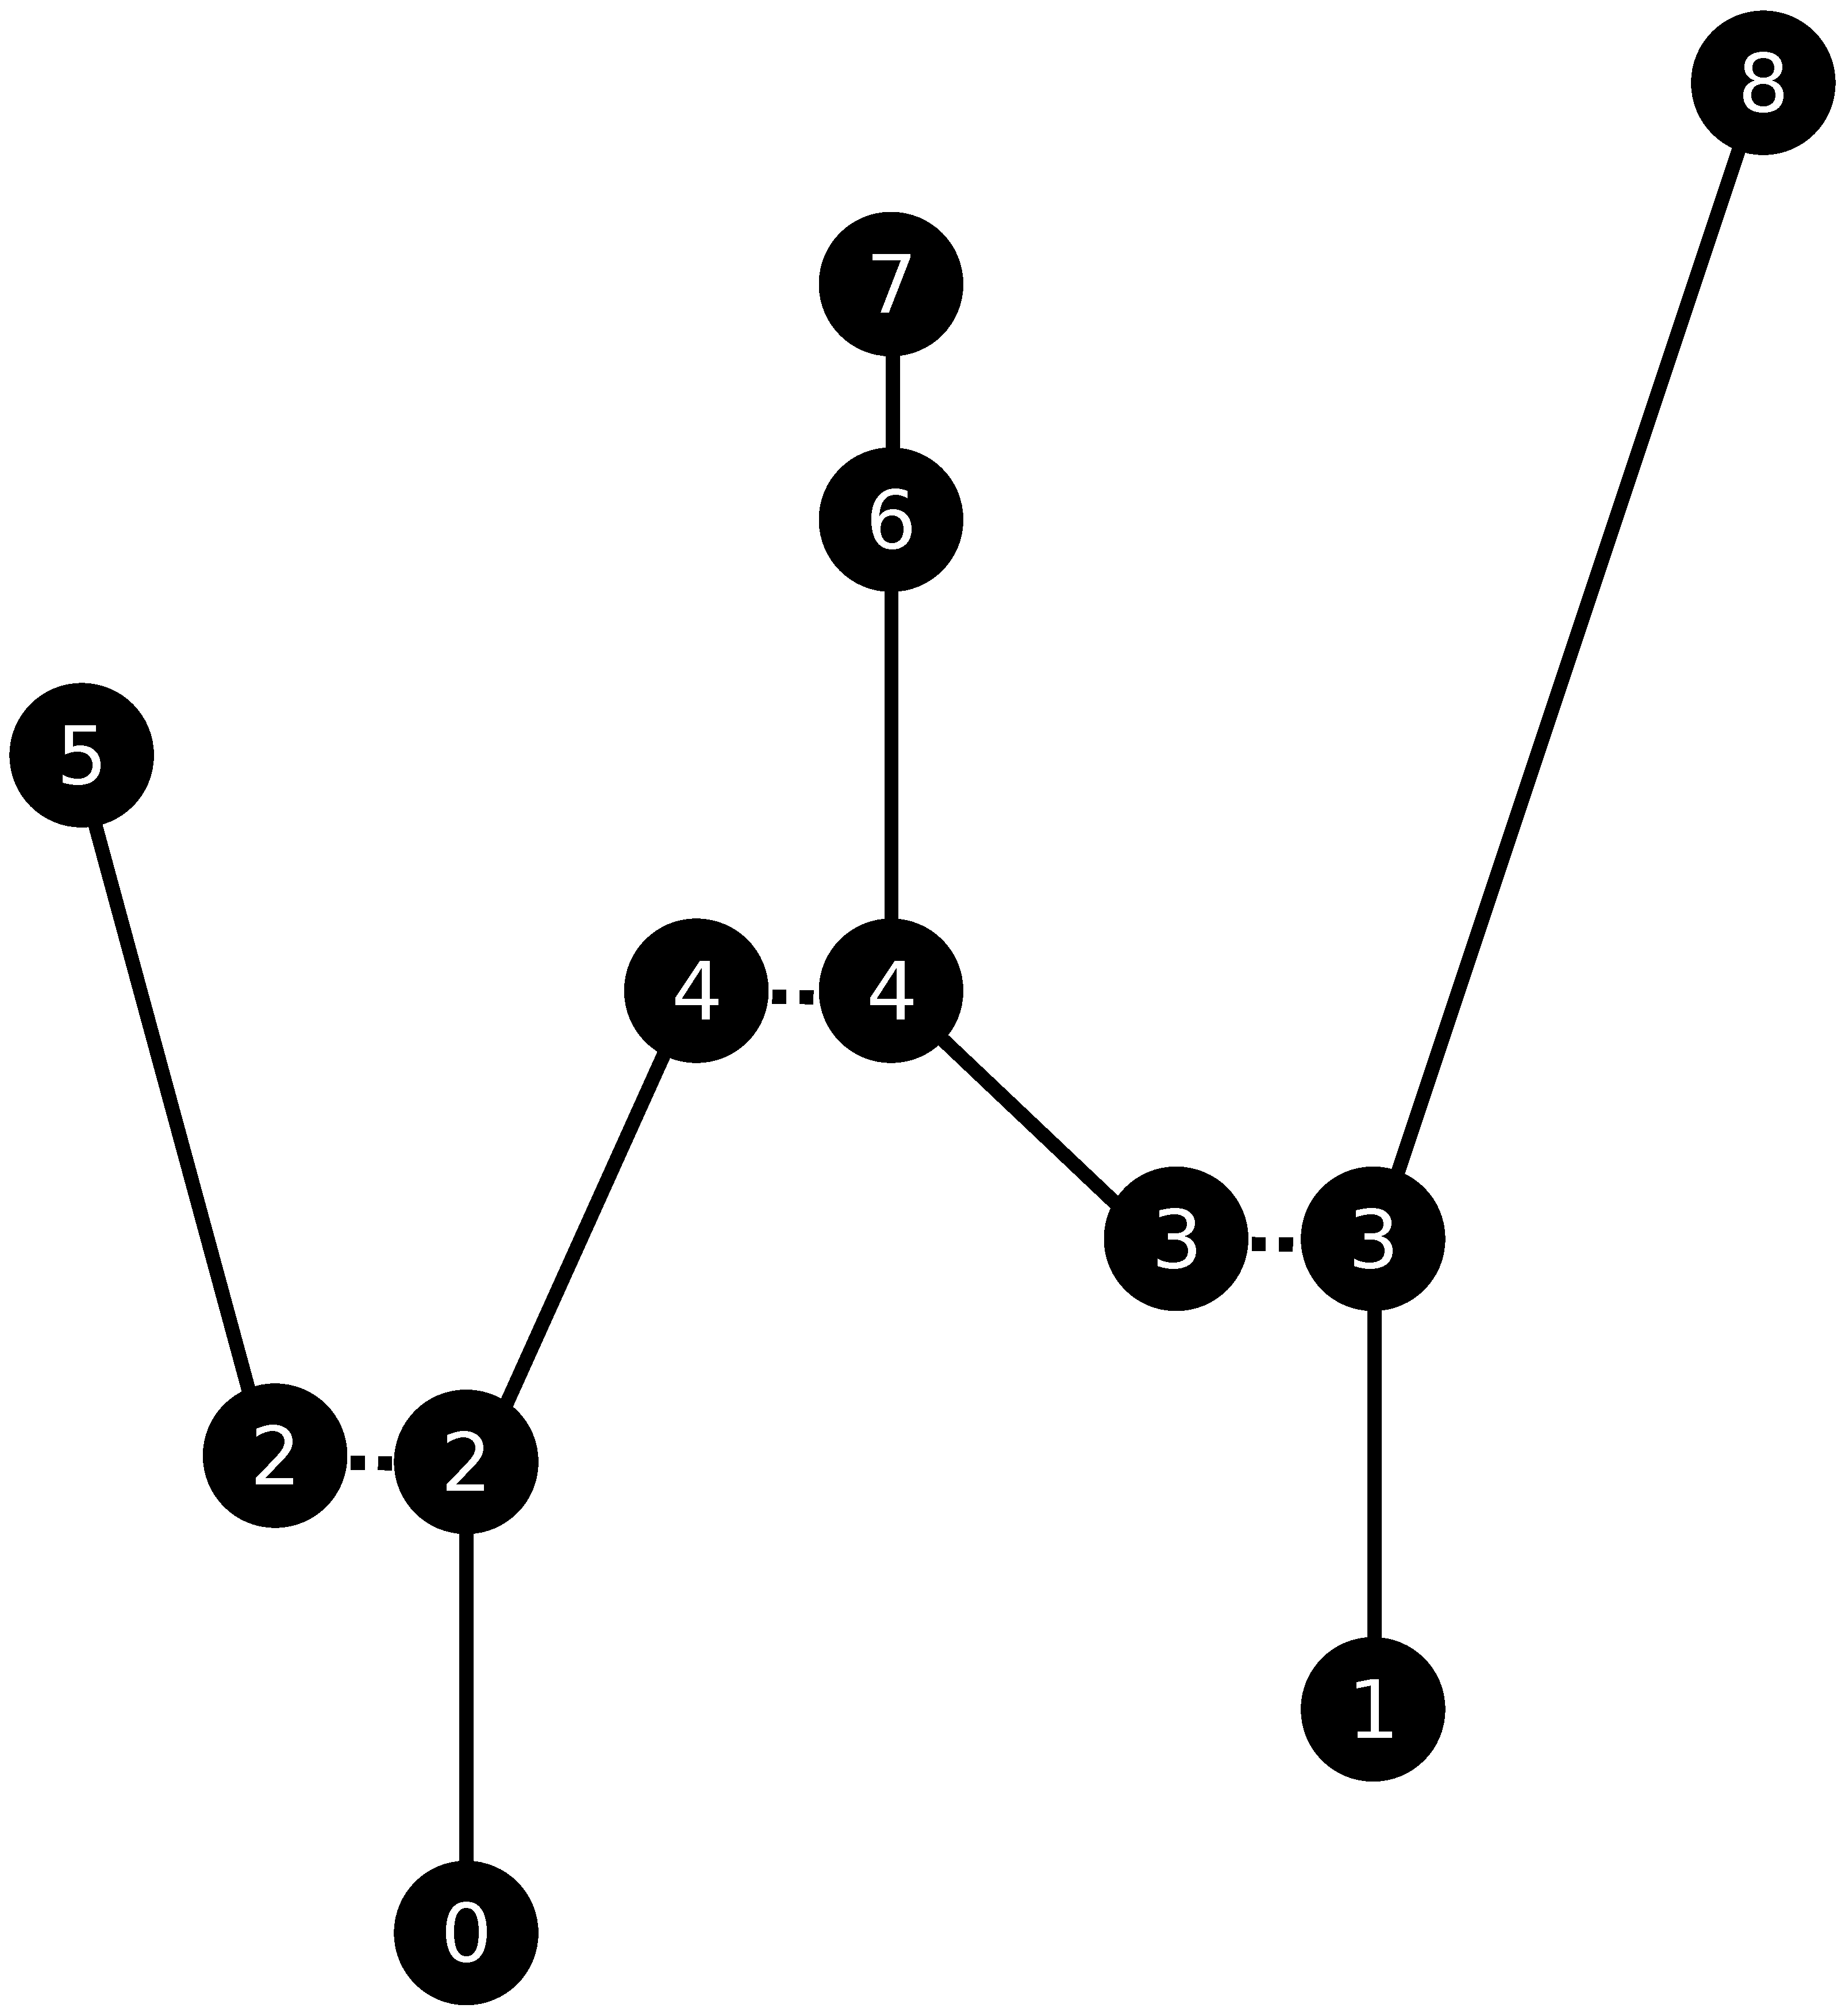
\includegraphics[scale=0.11]{./images/w3x3-ct-decomp.eps}}}%
    \subfloat[Heirarchical view of the branches.]{{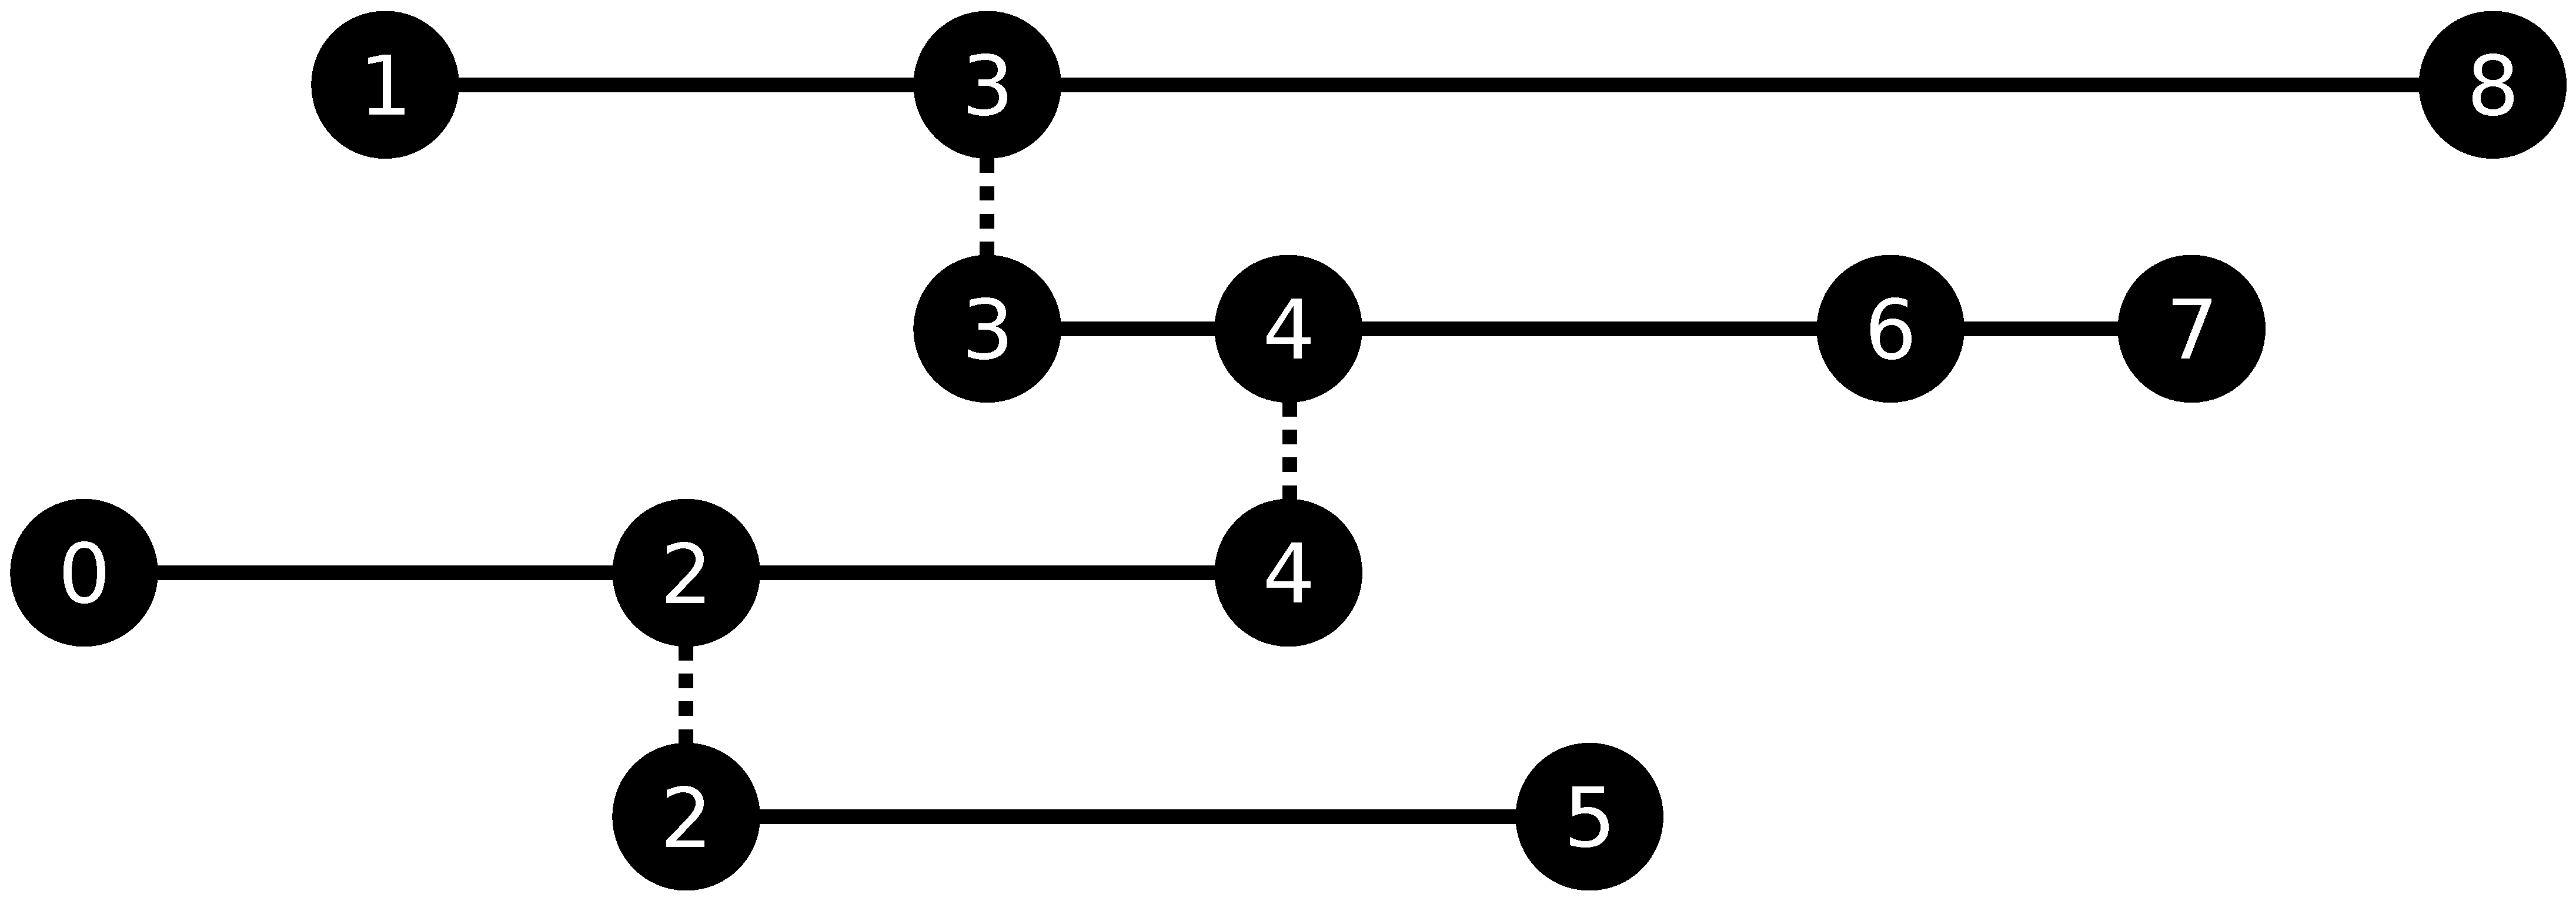
\includegraphics[scale=0.11]{./images/w3x3-ct-h-decomp.eps}}}%
    \caption{Branch Decomposition of the Contour tree from Figure \ref{fig:mesh-join-split-contour} [which subfigure?].}%
    \label{fig:branch-decomp}%
\end{figure}

Branch decomposition is a form of topological simplification whose use is limited to the contour trees. In Chapter 6 we will present a more general topological simplification framework called persistent homology. Our goal will be to express branch decomposition in the framework of persistent homology and determine whether the two are equivalent.

% @TODO Todo talk about how this is used to remove noise and artifacts in data.

% @TODO Remove Stay Tuned
% The paper \cite{ct-branch-decomp} cites that the persistence defined in that way is similar to persistence first defined in \cite{persistence-original}. In Chapter N of this dissertation we will demonstrate that this claim is either incorrect of misleading. Stay tuned folks.
